\documentclass{article}
\usepackage{ctex}
\usepackage{hyperref}

\begin{document}

\title{周报}
\author{刘精昌}
\maketitle

\section*{本周工作}
\begin{enumerate}
  \item 看了《Distributed Multi-Task Learning with Shared Representation》,主要关于分布式多任务学习。《An Empirical Study of ADMM for Nonconvex Problems》NIPS16 opt workshop,较短,主要是ADMM相关实验结果。
  \item 课程作业、复习备考相关。
\end{enumerate}

对于《Distributed Multi-Task Learning with Shared Representation》这篇paper,比较了一些用来解决MTL分布式优化问题,如图\ref{1} 所示。
\begin{figure}
  \centering
  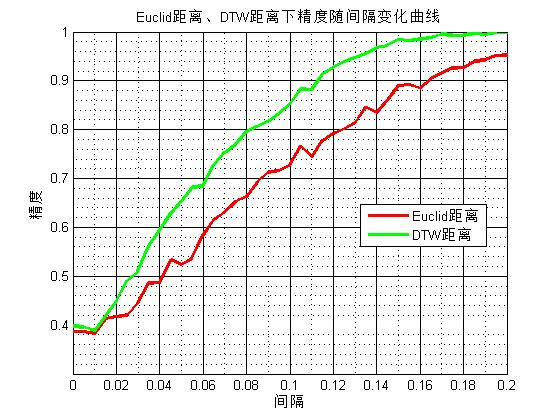
\includegraphics[width=\textwidth]{1.png}
  \caption{MTL分布式优化问题的比较}\label{1}
\end{figure}

Samples这一列表示为了达到 $\epsilon$ 的精度,每个worker需要的采样数目,牵扯到learning theory中的PAC学习。Communication这一列表示迭代的每轮中,通信次数。ERM表示workers在该算法中做经验风险最小化的工作,Gradient Comp表示worker做的是计算梯度的工作。

\section*{下周计划}
\begin{itemize}
    \item 看其他关于SGD改进文章。
    \item 看看周师姐今天报告的第二篇paper,考虑能不能在View learning中,考虑多个View 的情况。 以及放松对views之间条件独立的assumption,对相关设置个容忍度。
    \item 花时间应对考试。
\end{itemize}
\end{document} 